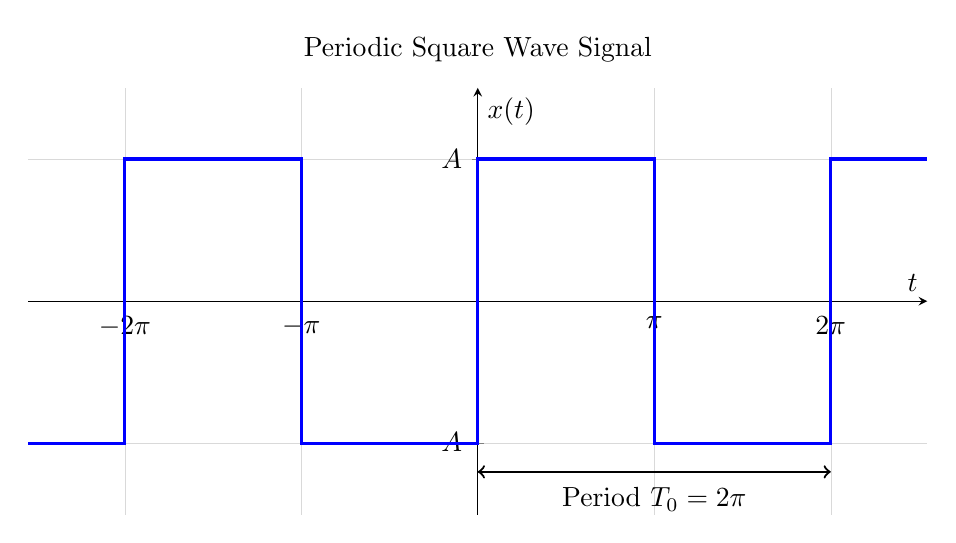
\begin{tikzpicture}
	\begin{axis}[
		width=13cm,
		height=7cm,
		axis lines=middle,
		xlabel={$t$},
		ylabel={$x(t)$},
		title={Periodic Square Wave Signal},
		xmin=-8, xmax=8,
		ymin=-1.5, ymax=1.5,
		xtick={-6.28, -3.14, 3.14, 6.28},
		xticklabels={$-2\pi$, $-\pi$, $\pi$, $2\pi$},
		ytick={-1, 1},
		yticklabels={$-A$, $A$},
		grid=major,
		grid style={line width=.1pt, draw=gray!30},
		no marks,
		]
		
		% Use 'const plot' for a cleaner way to draw square waves
		\addplot[const plot, blue, very thick] coordinates {
			(-8, -1)
			(-6.283, 1)
			(-3.141, -1)
			(0, 1)
			(3.141, -1)
			(6.283, 1)
			(8, 1)
		};
		
		% Add a single, correct period marker
		\draw[<->, thick] (axis cs:0, -1.2) -- (axis cs:6.283, -1.2) node[midway, below=2pt] {Period $T_0 = 2\pi$};
		
	\end{axis}
\end{tikzpicture}